	
	
	
	
сервери, на яких більша частина памʼяті є вільною
сервери, які могли б цю памʼять використовувати, якщо мали би до неї доступ
	Програмне забезпечення першого типу зазвичай має “вузьке місце” у ресурсах процесору (наприклад, виконує задачі кодування даних, або простого обміну даними), програмне забезпечення другого - у ресурсах памʼяті (зазвичай це аналіз великих масивів даних або просто у програмного забезпечення є деякий великий набір даних, який йому потрібен для роботи). Використання памʼяті диску для розширення основної памʼяті не є оптимальним - через великий час доступу (а в хмарній інфраструктурі в додаток до цього зазвичай диски не є локальними, а розміщені віддалено на локальній інфраструктурі). У порівнянні з часом доступу до диску час доступу до даних у памʼяті іншого серверу є значно меншим (хоча все ще більшим за той випадок, коли дані доступні локально).

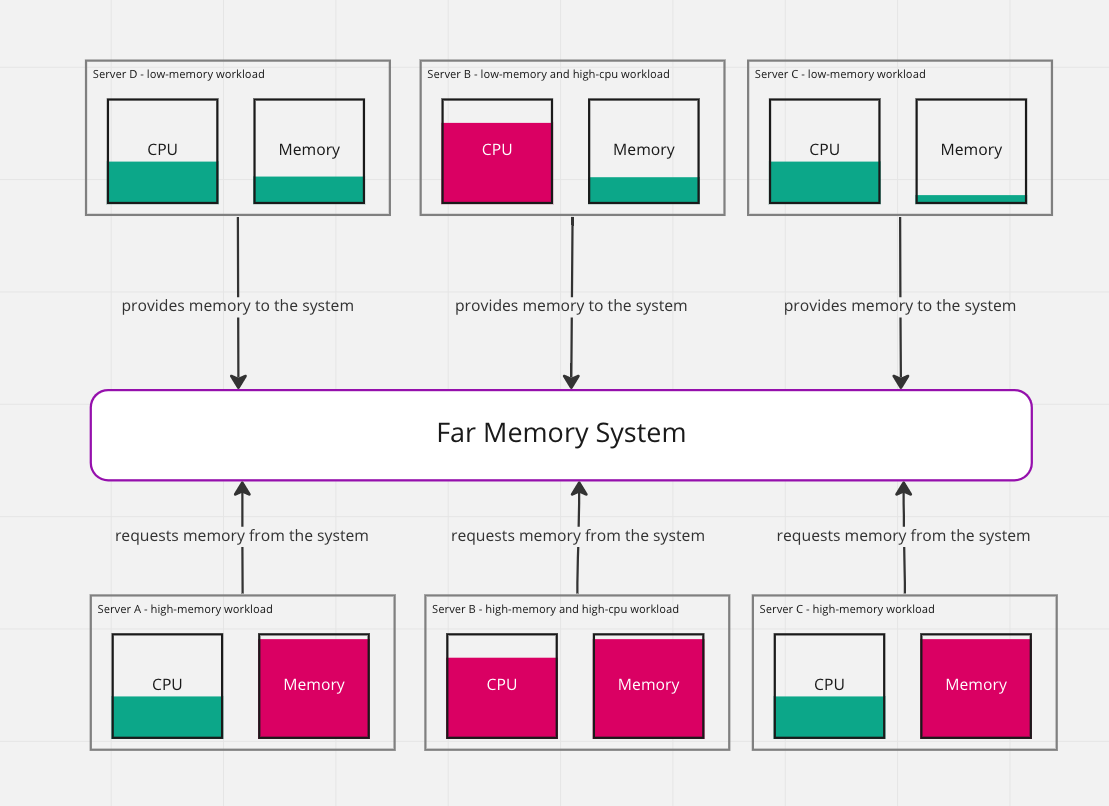
\includegraphics[width=5cm, height=4cm]{image1.png}
Рисунок 1.1 - Схематичне зображення принципу роботи Far Memory.
Це все робить використання такої віддаленої памʼяті привабливим для випадків, коли можна знайти сторінки памʼяті, доступ до яких відбувається порівняно не часто, перемістити їх у віддалену памʼять та звільнити місце для даних, доступ до яких відбувається частіше.

\section{Аналіз існуючих реалізацій віддаленої памʼяті}

Аналіз існуючих реалізацій віддаленої памʼяті має на меті проаналізувати існуючі реалізації, їх архітектуру, причини певних рішень. Ціллю є дізнатися які з вже досліджених підходів є ефективними та знайти відповіді на наступні дослідницькі питання:
З яких компонентів складаються системи віддаленої памʼяті, що працюють в розподілених системах?
Яким чином вони інтегруються в існуюче та нове програмне забезпечення?
Що впливає на швидкодію системи та які є методи її покращення?
За рахунок чого забезпечується відмовостійкість?
Відповіді на ці питання дозволять коректно розробити архітектуру рішення, що розглядається в межах цього курсового проекту, уникнути можливих помилок.

\subsection {Remote Direct Memory Access та її реалізації}

Технологія віддаленого прямого доступу до памʼяті (Remote Direct Memory Access) полягає в використанні спеціальних апаратних засобів, що дозволяють вузлам в системі отримувати дані з інших вузлів з невеликою затримкою з інших вузлів без витрачання ресурсів процесору цих вузлів для обробки запитів. Однією з найбільш розповсюджених реалізацій RDMA є InfiniBand. Цей підхід використовується і є виправданим для використання в середовищах високопродуктивних обчислень (High Performance Computing - HPC). Головним недоліком цієї реалізації віддаленої памʼяті є те, що вона потребує додаткового спеціалізованого обладнання. Для задач та середовища що розглядаються в цьому курсовому проекті не є підхожим рішенням, тому що використання використання додаткових пристроїв потребує додаткових ресурсів і не вирішує проблему більш ефективного використання наявних ресурсів без змін в апаратну платформу.

\subsection {Software-Defined Far Memory in Warehouse-Scale Computers}

    Компанія Google розробила та в тестовому режимі інтегрувала систему віддаленої памʼяті в своїх центрах обробки даних. Наскільки відомо на момент проведення дослідження існуючих реалізацій для цього курсового проекту, це єдиний великий оператор центрів обробки даних, який спроектував та застосував систему віддаленої памʼяті на великих масштабах та обладнанні яке виконує програмне забезпечення, що обробляє запити від користувачів (іншими словами, на справжньому навантаженні, а не у тестовому середовищі).
	В науково-дослідній роботі, опублікованій Google, зазначається що система для своєї роботи використовує функціонал ядра операційної системи Linux під назвою zswap. Перевагою такого рішення є те, що zswap це перевірена часом технологія, яка надає можливість компресії сторінок памʼяті. Інтеграція з цим функціоналом дозволяє переносити частини памʼяті на віддалені вузли без використання додаткового апаратного забезпечення.
Система відслідковує час останнього доступу до сторінок памʼяті для визначення “холодних” сторінок, які було б ефективно перенести у віддалену памʼять. Також окремий компонент системи відслідковує сторінки, які потрібно перенести з віддаленої памʼяті у локальну. Обидва з цих компонентів контролюються встановленим на кожен сервер агентом віддаленої памʼяті. Ця програма збирає статистику використання памʼяті та задає параметри роботи для системи.
В публікації зазначено, що режими доступу до памʼяті постійно змінюються. Наприклад, зібрана статистика показує що кількість холодних сторінок памʼяті варіюʼться від 1% до 61% в залежності від часу дня, програмного забезпечення що розгорнуто на серверному обладнанні, запитів від користувачів та конкретного серверу. Це створює необхідність мати окремий компонент автоматичного налаштування системи. Цей компонент отримує статистику зібрану агентами на обчислювальних вузлах та за допомогою моделей машинного навчання обирає нові значення параметрів для компонентів що керують переміщенням сторінок памяʼті.
Недоліком системи є те, що її програмний код не є публічно доступним, а окремі компоненти є специфічними для середовища, що використовується в компанії Google.

\subsection{Carbink: Fault-Tolerant Far Memory}

Carbink це також система віддаленої памʼяті розроблена та протестована компанією Google в своїх центрах обробки даних. Ця реалізація фокусується на покращені відмовостійкості та зниженні рівня затримок при роботі з віддаленою памʼяттю.
Важливим компонентом цієї реалізації є менеджер памʼяті (memory manager). Цей компонент керує розподілом фрагментів памʼяті по вузлах, що їх зберігають та перевіряє стан роботи цих вузлів. Важливим припущенням є те, що вважається що менеджер памʼяті завжди залишається в робочому стані. Мережевий звʼязок теж вважається стабільним.
Відмовостійкість забезпечується тим, що коли менеджер памʼяті виявляє недоступність одного з вузлів памʼяті (через апаратний чи програмний збій), то запускається процес відновлення. Завдяки використанню методу кодування з видаленням (erasure coding) при втраті блоку даних з одного вузла, його можна відновити за допомогою певних математичних перетворень інших даних. Перевагою такого методу є невеликий рівень надлишковості у порівнянні з рішенням, яке використовує реплікацію (тобто зберігання декілька копій даних).
Низька затримка забезпечується головним чином за допомогою обʼєднання невеликих шматків даних у більш великі (розміром декілька мегабайт) блоки (які називаються spans). Робота з більш великими блоками знижує навантаження на мережу та час для отримання даних. Недоліком такого підходу зазначається зберігання зайвих даних у блоках, що приводить до дещо більшого (на 35%) використання памʼяті на віддалених вузлах.
Для інтеграції з клієнтським програмним забезпеченням (в якого є потреба у додатковій памʼяті) використовується бібліотека написана на мові C++ що дає доступ до памʼяті за допомогою розумних покажчиків. Це вимагає деякої зміни в програмне забезпечення.
Аналогічно до попередньої системи, програмний код для цієї реалізації не є публічно доступним. Це не дозволяє використати систему в центрах обробки даних інших операторів.

\subsection{AIFM: High-Performance Application-Integrated Far Memory}

Система Application-Integrated Far Memory була розроблена дослідниками з VMWare Research. У порівнянні з реалізаціями віддаленої памʼяті компанії Google, ця система має схожі та відмінні елементи.
	Головною відмінною рисою цієї реалізації є інтеграція з клієнтським програмним забезпеченням за допомогою клієнтської бібліотеки на C++ що надає розумні покажчики та структури даних оптимізовані для використання з віддаленою памʼяттю.
	Для спілкування між сервером що надає памʼять та сервером що її потребує використовується TCP/IP зʼєднання.
	Для виявлення ділянок памʼяті, що можна перенести у віддалену памʼять, використовується механізм відслідковування рівня гарячесті сторінок памʼяті. Також, для підвищення ефективності, структури даних визначені бібліотекою AIFM реалізують предзванатжання наступних ділянок памʼяті.
	Для цієї реалізації є доступним програмний код. Недоліком є те, що без додаткової доробки він підтримує лише один сервер що надає віддалену памʼять. Система не містить компоненту для розподілення та керування памʼяттю по кластеру вузлів. Також реалізація не є придатною для розгортання в середовищах що обробляють справжнє навантаження без додаткової доробки. Система має складний процес розгортання, залежить від зовнішніх компонентів, не має простих механізмів конфігурування та моніторингу.

\section{Відповіді на дослідницькі питання}

За результатами аналізу існуючих реалізацій віддаленої памʼяті було знайдено відповіді на питання поставлені на початку роботи.
	Системи віддаленої памʼяті, що працюють у розподілених системах, містять клієнтський компонент, роль якого полягає в наданні доступу клієнтському програмному забезпеченню до віддаленої памʼяті. Основними способами реалізації такого компонента є створення окремого сервісу що працює поряд з іншим навантаженням на тому ж обладнанні та інтеграція якого відбувається засобами операційної системи. Перевагою такого методу є відсутність необхідності вносити зміни в існуюче програмне забезпечення, що робить інтеграцію системи віддаленої памʼяті більш простою задачею для операторів центрів обробки даних. На відміну від цього, іншим поширеним рішенням є інтеграція на рівні програмного забезпечення завдяки використання спеціальної бібліотеки, що надає доступ до віддаленої памʼяті з використанням розумних покажчиків та спеціалізованих реалізацій структур даних. Цей метод в вивчених дослідженнях показав більш високу ефективність. Крім цього, задачами що вирішує клієнтський компонент є визначення умов за яких фрагменти памʼяті вважаються холодними та переміщення їх у віддалену памʼять та завантаження з неї. Крім цього цей компонент повинен збирати статистику, яка аналізується для автоматичної зміни налаштувань системи.
	Оскільки відаленна памʼять розміщена на великої кількості віддалених вузлів, то виникає необхідність використання центрального компонента, який є площиною управління для кластеру. Роль такого компонента зазвичай полягає в розподілені фрагментів памяʼті по кластеру та обробка ситуацій коли потрібно виконати міграцію даних (у разі запланованого виходу вузлів з кластеру) чи відновлення даних (у разі апаратного чи програмного збою на вузлі кластеру). Цей компонент підтримує звʼязок з усіма іншими компонентами системи.
	Сервіс зберігання даних є також невідʼємною складовою будь-якої реалізації віддаленої памʼяті. В усіх вивчених реалізаціях цей компонент має інтерфейс читання та запису фрагментів памʼяті за ключем та використовується або площиною управління та/або клієнтськими реалізаціями.
	Компонент автоматичного налаштування системи є опціональним, але здатним помітно підвищити ефективність (тобто знизити затримки операцій) віддаленої памʼяті. Це зазначено в деяких з існуючих реалізацій, що вивчались.

\section{Постановка задачі}

Метою роботи є покращення інфраструктурних компонентів та інструментів, що можуть використовуватись операторами центрів обробки даних та розробниками програмного забезпечення для розгортання та використання віддаленої памʼяті. Для досягнення мети необхідно вирішити наступні задачі:
аналіз технічних рішень, що використовуються в існуючих реалізаціях, особливостей програмних та апаратних платформ, що використовуються для розгортання сучасного програмного забезпечення.
розробка методу та архітектури програмного забезпечення для надання програмно-визначеної віддаленої памʼяті у розподілених системах
реалізація програмного забезпечення для надання віддаленої памʼяті а також необхідні компоненти для інтеграції його у клієнтське програмне забезпечення згідно з розробленою архітектурою.
оцінка ефективності запропонованого рішення.
Створене програмне забезпечення повинно відповідати наступним вимогам:
Реалізація віддаленої памяʼті повинна містити сервіс, який користувачі системи можуть розгорнути на вузлах системи (під управлінням операційної системи Linux), що мають вільну памʼять для її використання по мережі. Цей компонент повинен використовувати невелику кількість ресурсів, та для зберігання даних використовувати кількість памʼяті задану користувачем або визначену автоматично.
Реалізація повинна мати варіанти інтеграції як в нове програмне забезпечення (де є можливість змінювати програмний код) так і в існуюче (де змінювати код не є можливим).
Для вирішення проблеми, що розглядається, затримка системи в операціях читання та запису повинна бути нижчою за затримки при зберіганні даних у постійному сховищі, таких як жорсткі диски та твердотільні накопичувачі, що є доступними у середовищах де ця система буде розгортатися.
Повинен бути наявний центральний компонент, який налаштовує конфігурацію та дозволяє керувати усією системою.
Реалізація повинна мати автоматичну зміну параметрів з урахуванням особливостей програмного забезпечення, що використовується.
Повинна забезпечуватись відмовостійкість та збереження даних що зберігаються у разі апаратних чи програмних збоїв у кластері.
Програмне забезпечення повинне бути простим у розгортанні,  адмініструванні а також у інтеграції в клієнтське програмне забезпечення.
	Призначенням цієї розробки є надання компонентів для розгортання кластеру віддаленої памʼяті та інструментів для її використання в існуючому та новому програмному забезпеченні.

\section{Висновки}

У цьому розділі виконано аналіз проблеми та тематичних джерел за темою дослідження, що розглядається в цьому курсовому проекті. Було вивчено з яких складових частин складаються існуючі реалізації та як вони співпрацюють. З існуючих досліджень було інформацію про ефективність та недоліки підходів у архітектурі та керуванні віддаленої памʼяті. Інформація отримана в даному розділі буде використовуватись для розробки архітектури та реалізації програмного рішення, що розглядається у межах цього курсового проекту. В результаті проведеного аналізу сформульована постановка задачі, наведене призначення цілі та задачі розробки.

\chapter{Розробка архітектури програмно-визначеної віддаленої памʼяті}

\section{Компоненти системи}

З урахуванням специфіки доменної області, вимог, що висуваються до програмного забезпечення та результатів попереднього аналізу проблеми було розроблено архітектуру, що складається з наступних компонентів:
Сервіс зберігання блоків памʼяті
Сервіс керування кластером віддаленої памʼяті
Клієнтська інтеграція
	Центральна сутність, з якою працюють усі компоненти це блоки памʼяті.
	Усі компоненти програмного рішення віддаленої памʼяті розгортатимуться за допомогою бінарних виконуваних файлів призначених для операційної системи Linux, а також (за вибором користувача) з використанням Docker контейнерів, що можна розгорнути за допомогою сучасних систем оркестрації, як наприклад Kubernetes.
	Архітектура програмного рішення віддаленої памʼяті має наступні припущення щодо середовища, в якому вона буде розгортатися:
Вважається, що усі вузли системи розміщені у межах одного центру обробки даних та мають низькі мережеві затримки при спілкуванні між собою.
Мережа працює стабільно і між будь-якими двома вузлами в кластері є можливість встановити зʼєднання. Оскільки в багатьох інших задачах існує таке саме припущення (наприклад, у розподілених базах даних) і враховуючи той факт, що у межах одного центру обробки даних мережа зазвичай достатньо стабільна, то використання цього припущення не повинно накладати значних обмежень на середовища, в яких це програмне рішення може використатися.
Будь-яка розгорнута клієнтська інтеграція має можливість підключитися до сервісу керування кластером за призначеною йому IP адресою в мережі та номером порту.
Будь-яка розгорнута клієнтська інтеграція, а також сервіс керування кластером мають можливість підключитись до будь-якого розгорнутого сервісу зберігання блоків за призначеними їм IP адресами в мережі та номером порту.
Будь-який розгорнутий сервіс зберігання блоків даних має можливість відкрити зʼєднання з сервісом керування кластером за призначеною йому IP адресою в мережі та номером порту.
	Конфігурація усієї системи знаходиться та редагується користувачем в сервісі керування кластером віддаленої памʼяті. Для налаштування та додавання у кластер нової клієнтської інтеграції чи сервісу зберігання даних користувачу достатньо вказати IP адресу та порт сервісу керування кластером.
	Для реалізації усіх компонентів системи використовується мова програмування Rust.

\section {Блоки памʼяті}

Блоками памʼяті в цьому програмному рішенні є набором байт, які обробляються системою як єдина одиниця. Розмір блоку складає 4 мегабайти за замовчуванням або розмір вказаний користувачем при розгортанні системи. Як і в деяких існуючих реалізаціях, ціль використання блоків полягає в обʼєданні невеликих фрагментів памʼяті у більш великі блоки для більш швидкої та ефективної обробки, зниження затримки в операцій читання та запису.
	Кожному блоку памʼяті призначається унікальний ідентифікатор (ID), який є цілим числом, яке займає 64 біти памʼяті.

\section {Cервіс зберігання блоків}

Сервіс зберігання блоків - сервіс, що розгортається на вузлах розподіленої системи, що містять вільну памʼять для надання доступу до неї по мережі.
	Інтерфейсом цього компоненту є сховище ключ-значення, де ключем є ідентифікатор блоку памʼяті, а значенням - байти блоку.

\section {Сервіс керування кластером}

Сервіс керування кластером приймає від розгорнутих сервісів зберігання блоків інформацію про кількість блоків, яку вони можуть отримати для зберігання. Далі, за запитами від клієнтських інтеграцій, сервіс керування кластером призначає їм ідентифікатори блоків для використання в клієнтському програмному забезпеченні, а також адреси сервісів зберігання блоків, на яких вони розміщені.
	Для забезпечення відмовостійкості, користувач обирає один зі способів забезпечення відновлення даних у разі програмних чи апаратних збоїв:
Реплікація (за вказаним користувачем фактором n) - цей алгоритм створює n ідентичних копій даних на різних вузлах системи. У разі якщо один з вузлів вийде з кластеру, то дані будуть відновлені з інших вузлів, де зберігаються репліковані копії.
Кодування стиранням (erasure coding) - цей алгоритм ділить блоки даних на менші блоки, кожен з яких має надмірність (конфігурація алгоритму задається користувачем в залежності від його вимог до відмовостійкості кластеру). У разі відмови одного з вузлів кластеру, втрачену інформацію можна відновити з інших частин виконавши нескладні математичні перетворення.
Сервіс керування кластером також надає інструменти для моніторингу, перегляду стану компонентів та внесення змін в кластер. Надається веб-інтерфейс користувача для перегляду інформації. Для інтеграції з зовнішньою системою моніторинга надається HTTP інтерфейс для передачі метрик та статистики у форматі Prometheus.
Крім цього, на сервісі керування кластером полягає роль автоматичної зміни конфігурації кластеру на основі статистики зібраної клієнтськими інтеграціями. Ці налаштування мають вид правил, які відправляються на клієнтські інтеграції та задають їм за яких умов необхідно виконати предзавантаження окремих блоків даних для зниження часу затримки.

\section {Клієнтська інтеграція}

Як зазначалось раніше, клієнтська інтеграція має два варіанти для розгортання на вибір користувача (в кластері можно використовувати обидва одночасно).

\subsection{Бібліотека на мові програмування Rust для інтеграції в клієнтське програмне забезпечення}

Цей спосіб використання підходить для програмного забезпечення, код якого є можливість змінити та яке написане на мові програмування Rust. Ця інтеграція є рекомендованою для використання, оскільки більш ефективна в роботі та має більш низькі затримки.
	Для її використання, користувач додає в своє програмне забезпечення бібліотеку, яка надає йому наступні інструменти для використання в своєму коді:
Розумний показчик FarMemory<T>, який за допомогою механізмів Deref<T> та Drop<T>, наданих мовою програмування Rust, завантажує дані та відправляє до віддаленою памʼяті за необхідністю.
Структура даних FarMemoryList<T> яка реалізує інтерфейс списку та зберігає дані у віддаленій памʼяті
Структура даних FarMemoryTable<K, V> яке реалізує інтерфейс хеш-таблиці та зберігає дані у віддаленій памʼяті
Функцію allocate\textunderscore far\textunderscore memory\textunderscore block, яка резервує блок у віддаленій памʼяті та повертає його ідентифікатор. Ця функція призначена для випадків коли розробнику потрібен низькорівневий доступ до памʼяті.
Функції read\textunderscore far\textunderscore memory\textunderscore block та write\textunderscore far\textunderscore memory\textunderscore block що дозволяють прочитати та записати зміст блоку у віддаленій памʼяті за його ідентифікатором. Ці функція призначена для випадків коли розробнику потрібен низькорівневий доступ до памʼяті.
Функція free\textunderscore far\textunderscore memory\textunderscore block, що визволяє з використання блок памʼяті за його ідентифікатором. Ця функція призначена для випадків коли розробнику потрібен низькорівневий доступ до памʼяті.

\subsection {Сервіс клієнтської інтеграції}

Цей варіант використання призначено для випадків, коли немає можливості змінити програмний код клієнтського програмного забезпечення, або коли воно використовує інші мови програмування, що не дозволяє використати бібліотеку клієнтської інтеграції.

Цей спосіб полягає в розгортанні сервісу на тому ж обладнанні, яке виконує програмне клієнтське програмне забезпечення. Сервіс використовує відповідний функціонал операційної системи Linux для створення віртуального блокового пристрою. Далі цей блоковий пристрій використовується клієнтським забезпеченням для прямого зберігання даних (за необхідністю, на блоковому пристрою розміщується файлова система) або на блоковому пристрою розміщується файл підкачки, в який операційна система при низькому рівні вільної памʼяті, автоматично переносить сторінки памʼяті.

\section {Взаємодія компонентів}

Для комунікації між компонентами використовується TCP/IP зʼєднання. Для кодування повідомлень має сенс використати Protocol Buffers. Це дозволить пересилати дані між компонентами з низькими затримками та додатковими витратами.

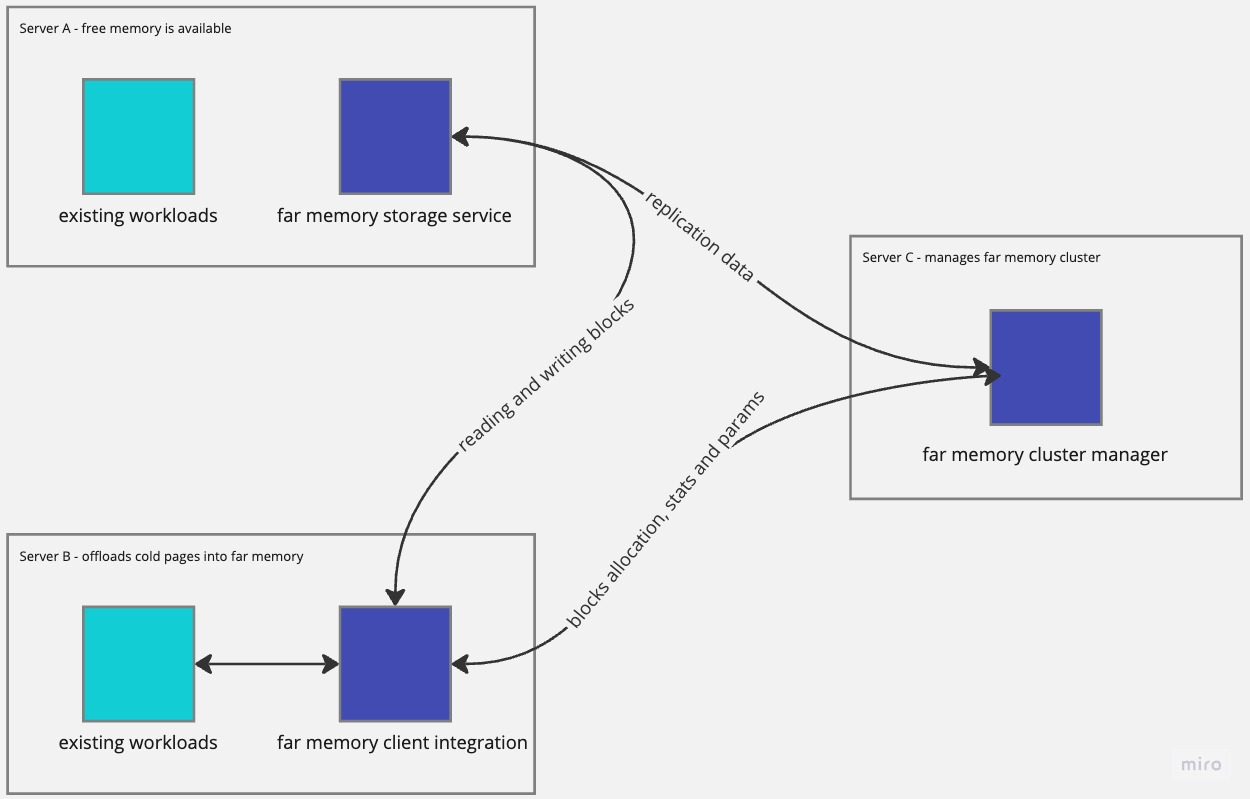
\includegraphics[width=5cm, height=4cm]{image2.jpg}

Рисунок 2.1 - Схема компонентів кластеру та потоки даних між ними.

\section{ВИСНОВКИ}

В цьому розділі було формалізовано вимоги до програмного рішення, що розглядається в межах цього курсового проекту. Грунтуючись на цих вимогах, було розроблено архітектуру програмно визначеної віддаленої памʼяті призначеної для розгортання у сучасних розподілених системах. Ця архітектура та описані деталі її реалізації будуть в подальшому використовуватись при реалізації, тестуванні та впровадженні цього програмного рішення.

\chapter{ВИСНОВОК}

Як підсумок проведеного аналізу проблеми, існуючих досліджень та реалізації та розробки архітектури архітектури програмного рішення програмно-визначеної віддаленої памʼяті, що розглядається у межах цієї роботи, було зроблено декілька висновків.
По-перше, реалізація кластеру віддаленої памʼяті повинна містити наступні компоненти: сервіс керування кластером, сервіс зберігання даних та клієнтська інтеграція. Ці компоненти пересилають блоки памʼяті мережею для переміщення холодних сторінок памʼяті у віддалену памʼять та у зворотному порядку.
По-друге, було встановлено, що найбільш оптимальним методом інтеграції в клієнтське програмне забезпечення є створення бібліотеки яка надає розробникам функції та структури даних для використання в своєму програмного забезпеченні. Також, оскільки велика частка програмного забезпечення не може змінюватись або не підходить до інтеграції з клієнтською бібліотекою за будь-яких причин, було досліджено та реалізовано у архітектурі альтернативний шлях реалізації: за допомогою віртуального блокового пристрою створеного за допомогою відповідного функціоналу операційної системи Linux.
По-третє, були визначені та додані в архітектуру засоби забезпечення відмовостійкості системи та низької затримки операцій читання та запису у віддалену памʼять.
В подальшому, розроблені вимоги та архітектура будуть використані для реалізації програмного рішення, його тестування та впровадження. 

\chapter {СПИСОК ВИКОРИСТАНИХ ДЖЕРЕЛ}

Software-Defined Far Memory in Warehouse-Scale Computers [Електронний ресурс] // Andres Lagar-Cavilla, Junwhan Ahn, Suleiman Souhlal, Neha Agarwal, Radoslaw Burny, Shakeel Butt, Jichuan Chang, Ashwin Chaugule, Nan Deng, Junaid Shahid, Greg Thelen, Kamil Adam Yurtsever, Yu Zhao, and Parthasarathy Ranganathan - International Conference on Architectural Support for Programming Languages and Operating Systems - 2019. Режим доступу до ресурсу: https://research.google/pubs/pub48551/
Carbink: Fault-tolerant Far Memory [Електорнний ресурс] // Yang Zhou Hassan Wassel Sihang Liu Jiaqi Gao James Mickens Minlan Yu Chris Kennelly Paul Jack Turner David E Culler Hank Levy Amin Vahdat - Proceedings of the 16th USENIX Symposium on Operating Systems Design and Implementation, Usenix - 2022. Режим доступу до ресурсу: https://research.google/pubs/pub51559/
AIFM: High-Performance, Application-Integrated Far Memory [Електронний ресурс] // Zhenyuan Ruan, MIT CSAIL; Malte Schwarzkopf, Brown University; Marcos K. Aguilera, VMware Research; Adam Belay, MIT CSAIL - 14th USENIX Symposium on Operating Systems Design and Implementation (OSDI 20) - 2020. Режим доступу до ресурсу: https://www.usenix.org/conference/osdi20/presentation/ruan
Block Device Driver [Електорнний ресурс] // Linux Kernel Teaching. Режим доступу до ресурсу: https://linux-kernel-labs.github.io/refs/heads/master/index.html
Understanding InfiniBand and RDMA [Електронний ресурс] // Red Hat Customer Portal. Режим доступу до ресурсу: https://access.redhat.com/documentation/en-us/red\textunderscore hat\textunderscore enterprise\textunderscore linux/8/html/configuring\textunderscore infiniband\textunderscore and\textunderscore rdma\textunderscore networks/understanding-infiniband-and-rdma\textunderscore configuring-infiniband-and-rdma-networks

\end{document}
